\begin{savequote}[75mm]
Either the rest of the world can't live like the developed world or we need, as a society, to think more about the technology of providing these services with less intensive use of at least certain  resources. We need to do a more diligent job of good housekeeping.
\qauthor{Thomas E. Graedel (1940- )}
\end{savequote}

\chapter{Quantifying Energy-Water Resource Usage}
\label{Chapter 3}

\newpage

\section{Quantifying Life-Cycle Energy-Water Resource Usage Efficiency}

\section{Life Cycle Assessment and Inventory Modeling}

Life-cycle assessment (LCA) is an environmental accounting framework that was developed to systematically quantify the material and energy inputs and outputs from a product, process, or system throughout all its stages of life. It uses a cradle-to-grave or, in some cases, cradle-to-cradle perspective, to evaluate the design processes as well as the entire supply chain associated with manufacturing, transportation, the use phase, and waste management \cite(Rebitzer2004). Practically, process based LCA analyses, which shall be the focus of the remainder of this discussion, incorporate two distinct modeling phases. The first involves the development of a Life-cycle Inventory model is a cumulative record of all of the materials and energy flows required to deliver a single functional unit of the product or process in question. The second, optional, phase of LCA analyses is the Life-cycle Impact Assessment (LCIA) component. An LCIA model attempts to translate the raw energy and material flows contained within the LCI into different categories of environmental impacts such as global warming potential, ocean acidification, freshwater eutrophication, etc. 

In the context of this discussion, one of the stated goals of this dissertation project was to quantify the energy-water usage efficiency of artificial groundwater recharge projects involving the reuse of treated municipal wastewater. In order to accomplish this goal custom LCI models will be developed for five case study regions in which the distribution networks responsible for transporting the treated wastewater for its point of origin, the WWTP, to its destination point of consumption, an artificial groundwater infiltration basin positioned at a designated destination location, upstream within the regional watershed. The raw data supporting the creation of each of these custom LCI models shall be derived from the UC Berkeley supported Web Water-Energy Sustainability Tool (WWEST). In each case study, the scope of this LCI modeling exercise shall be limited to the construction and operational requirements associated with the WWTP plant, the treated water distribution network, and the infiltration basin. This system boundary has been defined in such a way as to emphasize the dynamic contribution of the treated wastewater distribution to the LCI of a given functional unit of treated wastewater delivered to the sub-surface in the face of variable geographic context.

\section{Wastewater Treatment Processes}

The phrase wastewater treatment encompasses a wide variety of different processes and operational facilities depending upon: the quality of the influent water, the volume of the influent water, and the desired quality/end-use application for the treated effluent water. In the United States the operation of WWTPs are regulated at both the State and Federal levels. At the Federal level the principle regulatory agency is the United States Environmental Protection Agency (USEPA) and the principle regulatory program is the National Pollutant Discharge Elimination System (NPDES). According to the legal mandate of the NPDES, WWTP operators (as well as a wide variety of other entities) are required to apply, at regular time intervals, for discharge permits which provide them with the legal right to release waters containing limited concentrations of regulated pollutants into the environment. Also under this mandate, the USEPA is required to distribute these permits and enforce non-compliance with their terms.

Since the inception of the NPDES program, the USEPA has worked to make readily accessibly a centralized database of all registered permit holders within the United States. This database in interesting for the purposes of this project in that it contains spatially referenced information about the operational aspects of every operating WWTP in the U.S. Crucially, this information includes data on maximum daily permitted flow rates and total maximum daily loads that can be used to parameterize the type of process based LCI model facilitated by the WWEST tool.

In terms of their basic physical layout and operational requirements, WWTPs are typically constructed with a tiered layout; comprising primary treatment, secondary treatment, and sometimes, various so called tertiary processes. Both primary and secondary treatment are terms that come with narrow legal definitions and are implemented at nearly all WWTP plants handling municipal sewage discharges. Tertiary treatment processes are more loosely defined and encompass a suite of advanced treatment processes that are so costly that they tend to only be implemented at a minority of WWTP that are subject to a unique  circumstances in terms of influent pollutant loadings/composition or requirements associated with designed high purity effluent end-use applications.

Primary treatment encompasses processes and equipment dedicated to the physical separation of non-soluble waste constituents present in the influent wastewater stream. Within a WWTP, a number of distinct processes are often lumped together as being part of the primary treatment. For example, when water first enters the WWTP it is guided through a series of progressively refined grates to screen out bulk pollutants such as anthropogenic trash or natural plant and animal detritus. Following from this bulk screening phase, the water is guided into a series of settling basins where its movement is slowed to crawl to facilitate the settlement of suspended pollutant materials such as sediment. Due to the slow rate at which this settling process proceeds, the physical infrastructure which supports it can comprise a significant fraction of the overall footprint of a WWTP; particularly for those with high flow volume processing requirements.

Secondary treatment encompasses processes and equipment dedicated to the biological (and sometimes chemical) degradation of soluble waste constitutes present in the influent wastewater stream. In most municipal WWTP secondary treatment is accomplished through a passively aspirated, aerobic biological digestion reactors. In these reactors large colonies of bacterial species are cultivated on high surface area media using the organic components of the influent wastewater stream as a feedstock for the continued growth. At the end of their life cycle, the bacteria fall to base of the reactor tank and must be continuously removed in the form of a product known as activated sludge.

Tertiary treatment encompasses processes and equipment dedicated to the removal of soluble inorganic and some organic chemical species (including some viruses and pharmaceutical agents) present within the influent wastewater stream. At present, tertiary treatment processes are not mandatory for all WWTP facilities regulated under the NPDES program. In general, they tend to only be implemented at those specific locations in which a last and credible threat to public or environmental health has been identified and for which a targeted tertiary treatment process exists to address. In this way, mandates for tertiary treatment are typically instigated at the state or local level and done so on a case by case basis. Among the most common tertiary treatment processes include: reverse osmosis filtration, batch irradiation with ultra-violent light, the application of specialized chemical amendments, de-nitrification processes, and others.

For the purposes of this analysis and the customized LCI models which shall be constructed as part of the case study investigations, only primary and secondary treatment processes shall be included in the scope. This decision has been made to eliminate a substantial bias in the inventory models process flows that might be associated with a single specialized tertiary treatment procedure.  

\section{Water Distribution Infrastructure}

The immediate delivery and reuse of treated wastewater for various municipal and agricultural end-use applications is still a relatively new phenomenon. As such, the regulatory landscape surrounding such practices is still not well defined at the Federal level here in the United States. Consequently, what regulations due exist, typically have been enacted at the State and local levels, with the most advanced frameworks, unsurprisingly, existing in those states such as Florida, California, and Arizona where the popularity of reuse as viable alternative source of freshwater supply, has been surging in recent years.

In all of the locations within the United States for which solid regulatory frameworks surrounding reuse currently exist, there are strong constraints governing the use of existing water distribution infrastructure for the transportation of treated wastewater from its point of origin, the WWTP, to its point of end-use. These regulations, without exception, stipulate that treated wastewater, even if returned to a level of quality consistent with requirements for potable use, cannot be conveyed using existing distribution infrastructure carrying potable water for human consumption in municipal areas. Due to this regulatory constraint, all treated wastewater destined for some sort of municipal reuse must be carried through dedicated parallel distribution infrastructure. In California, this infrastructure is easily identified at locations where treated wastewater is being reused due to the bright purple color of all the pipes. This color encoding is meant to be a strong visual reminder that the water being carried within them has not been deemed, from a regulatory perspective, as being fit for direct human consumption. 

The requirement that treated wastewater, regardless of its standard of treatment and anticipated end use application, be transported using a separate parallel distribution network is expected to be a crucial factor in determining the overall life-cycle energy-water usage efficiency of large scale water reuse systems feeding into artificial groundwater recharge basins. The reasoning behind this expectation is based upon the interaction of the following two key factors. [1] Water is a dense material, and thus it is very energy intensive to transport it over long distances and against steep elevation gradients. [2] Artificial groundwater recharge basins typically require fairly large amounts of contiguous land area that are situated in fairly close proximity to highly developed urban and suburban communities. Municipal water resource management agencies are tightly constrained in terms of the operating budgets from which they are able to draw funds to procure new land holdings for the purpose of constructing artificial recharge basins. Thus, artificial recharge basins , primarily to economic constraints, are typically located fairly far afield from the WWTPs which feed them.
 
\section{WWEST Recycled Water Reuse Life Cycle Inventory Model}

The WWEST Recycled Water Reuse Life-cycle Inventory Model refers to an integrated life-cycle inventory database and modeling framework for understanding the environmental impacts of wastewater treatment and reuse processes that was developed by a team of academic researchers operating out of the University of California at Berkeley College of Engineering. The principal investigator behind the project is Dr. Arpad Horvath, Professor of Civil and Environmental Engineering, and a specialist in the environmental impact assessment of civil infrastructure systems. The lead researcher on the WWEST project is Dr. Jennifer Stokes, with the initial development work on the WWEST model being completed as part of her doctoral dissertation project.

The LCI database underlying the WWEST toolset contains process flow information for the manufacture and operation of equipment and facilities involved in the supply, treatment, and distribution of municipal wastewater for the purpose of non-potable reuse. \ref{fig:WWESTsystem} 
provides a schematic overview of the WWEST database model components and their respective input data sources.

    \begin{figure}[!h]
        \begin{center}
        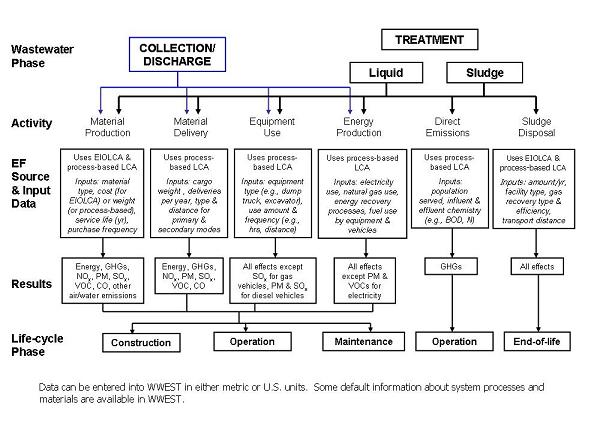
\includegraphics[width=5.5in]{figures/WWEST_System_Boundaries.jpg}
        \caption{WWEST Model System Boundaries}
        \label{fig:WWESTsystem}
        \end{center}
    \end{figure}
    
The WWEST LCI database can be accessed in two ways. The first, which provides full access to all of the attribute fields contained within the database, is via an excel spreadsheet that has been distributed with a built-in set of computational macros. The second method exposes a more limited range of the data values contained within the database and is accessible via a streamlined web application, also known as WWESTweb. The principle difference between the WWEST excel model and the web application is in the extent to which each allows the user to customize the various parameters associated with a hypothetic water reuse project and its supporting infrastructure. In this sense, the excel based model is more appropriate for building an LCI model to quantify the process flows attributable to an existing facility or which is in a very advanced stage of design planning. Conversely, the WWESTweb framework is more appropriate for less well defined scenario based planning exercises, where the primary goal is to assess the relative impact of major system design alternatives that have only roughly been fleshed out.

\section{WWEST Model Outputs}